\chapter{What Plants Need}\label{ch:g4:what-plants-need}

Two pots of cress stand on the same windowsill, sown the same
day. One is watered, one is not --- and within a week the
difference is written in green and yellow. With pots, \omterm{prop:g3:flowers-fruits-seeds:transform}{seeds} and
patience you can make \omterm{def:g1:plants-around-us:plant}{plants} themselves answer the question of
this chapter: what exactly does a \omterm{def:g1:plants-around-us:plant}{plant} need to live and grow?

\section{Asking plants questions: the fair test}

\begin{method}[The fair test]\label{met:g4:what-plants-need:fairtest}
To find out whether a \omterm{def:g1:plants-around-us:plant}{plant} needs something --- water, light,
soil, warmth:
\begin{enumerate}
  \item take \emph{two} pots of the same \omterm{def:g1:plants-around-us:plant}{plants}, sown the same
        way;
  \item treat them exactly alike in everything \emph{except the
        one thing tested} --- one gets it, the other does not;
  \item wait days or weeks, and compare;
  \item any difference must come from the one thing you changed:
        the test was fair.
\end{enumerate}
The untouched pot is called the \emph{control}\index{control
(experiment)}: it shows what happens when nothing is missing.
\end{method}

\begin{example}[Why two pots and not one]\label{ex:g4:what-plants-need:control}
Suppose a single unwatered pot wilts. Was it the missing water
--- or a cold snap, or bad \omterm{prop:g3:flowers-fruits-seeds:transform}{seeds}? With a watered twin standing
green beside it, grown from the same packet in the same room,
the doubt disappears: the twins differed in water alone.
One-pot experiments convince nobody, least of all a biologist.
\end{example}


\begin{omfigure}
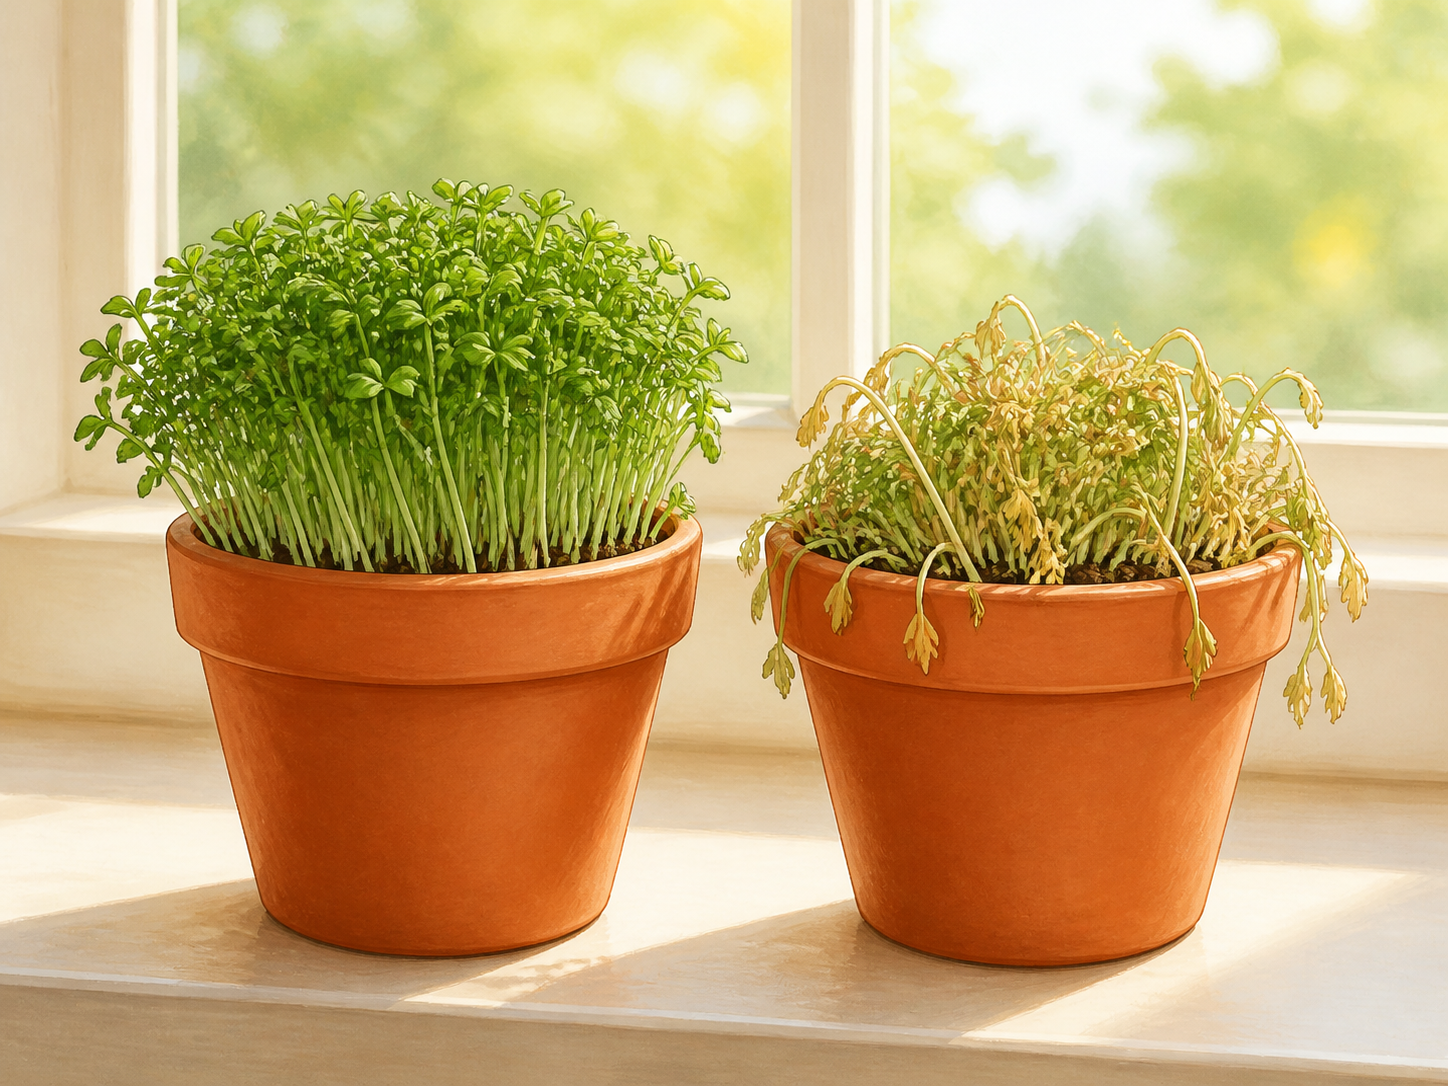
\includegraphics[width=0.58\linewidth]{images/book1/ai/g4-plants-cresspots.png}

{\small The same experiment on a real windowsill, one week in:
the twins now differ in everything visible --- because they
differed in one thing only.}
\end{omfigure}

\section{What the tests reveal}

\begin{proposition}[The needs of a plant]\label{prop:g4:what-plants-need:needs}
Fair tests, run for each need in turn, show that a \omterm{def:g1:plants-around-us:plant}{plant} needs:
\begin{itemize}
  \item \emph{water} --- the unwatered pot wilts and dies;
  \item \emph{light} --- the cupboard pot grows pale, long and
        weak, then gives up: no light, no \omterm{def:g1:plants-around-us:plant}{plant} food made;
  \item \emph{air} --- sealed away from fresh air, growth stops;
  \item \emph{warmth} --- in the cold, \omterm{prop:g3:flowers-fruits-seeds:transform}{seeds} wait
        (\cref{prop:g2:from-seed-to-plant:needs}) and growth
        freezes to a halt;
  \item \emph{mineral salts}\index{mineral salts}: tiny amounts
        of nourishing substances that the \omterm{def:g1:plants-around-us:parts}{roots} drink dissolved
        in the soil's water --- in pure water alone, a \omterm{def:g1:plants-around-us:plant}{plant}
        soon runs short.
\end{itemize}
\end{proposition}
\admitted

\begin{example}[The pale prisoner]\label{ex:g4:what-plants-need:pale}
The cupboard test of \cref{exo:g1:plants-around-us:8}, done
properly with a lit twin, gives a striking result: the prisoner
is not just sad but \emph{pale yellow} --- it stopped making its
green substance --- and strangely \emph{tall}, stretched out as
if searching for the missing light. Growth without light is
spending without earning; the \omterm{def:g2:from-seed-to-plant:seed}{seed}'s reserves once burnt, it
stops.
\end{example}

\begin{remark}[Why gardeners feed the soil]\label{rem:g4:what-plants-need:soil}
Compost and manure are not \omterm{def:g1:plants-around-us:plant}{plant} ``meals'' --- \omterm{def:g1:plants-around-us:plant}{plants} eat
nobody. They restock the soil's \omterm{prop:g4:what-plants-need:needs}{mineral salts}, which harvests
carry away year after year. The compost bin of
\cref{ex:g2:caring-for-nature:compost} closes the loop: what the
soil gave the vegetables, the peelings give back to the soil.
\end{remark}

\section{What plants do with what they take}

\begin{proposition}[Plants make their own matter]\label{prop:g4:what-plants-need:make}
\omterm{def:g1:animals-around-us:animal}{Animals} grow by eating other \omterm{def:g1:living-or-not:living}{living things}. A \omterm{def:g1:plants-around-us:plant}{plant} eats no one:
with water and \omterm{prop:g4:what-plants-need:needs}{mineral salts} from the soil, air, and the \omterm{prop:g3:balanced-diet:jobs}{energy}
of \emph{light} caught by its green \omterm{def:g1:plants-around-us:parts}{leaves}, it \emph{makes its
own matter} --- new \omterm{def:g1:plants-around-us:parts}{stems}, \omterm{def:g1:plants-around-us:parts}{leaves}, \omterm{def:g1:plants-around-us:parts}{roots} and \omterm{prop:g3:flowers-fruits-seeds:transform}{seeds}. That is why
light is food-and-drink serious for a \omterm{def:g1:plants-around-us:plant}{plant}, and why the green
\omterm{def:g1:plants-around-us:parts}{leaf} faces the sky.
\end{proposition}
\admitted

\begin{example}[A tree from almost nothing]\label{ex:g4:what-plants-need:tree}
\omterm{def:g1:plants-around-us:plant}{Plant} a pip in a large pot of weighed soil, wait years, and a
small tree stands there --- yet the soil has lost almost none of
its weight. The tree's wood was not scooped out of the pot: it
was \emph{made}, from water, air and light, in the green
workshops of the \omterm{def:g1:plants-around-us:parts}{leaves}. Where the matter of \omterm{def:g1:living-or-not:living}{living things} comes
from will keep us busy again in later years.
\end{example}

\begin{remark}[Green makes everyone's living]\label{rem:g4:what-plants-need:everyone}
Recall \cref{prop:g3:food-chains:start}: every \omterm{def:g3:food-chains:chain}{food chain} starts
with a \omterm{def:g1:plants-around-us:plant}{plant}. Now we see why that must be so --- \omterm{def:g1:plants-around-us:plant}{plants} are the
only link that makes new matter from non-living ingredients.
Every mouthful anyone eats, anywhere, was made in a \omterm{def:g1:plants-around-us:parts}{leaf} first.
\end{remark}

\section{Exercises}

\begin{exercise}[$\star$]\label{exo:g4:what-plants-need:1}
List the five needs of a \omterm{def:g1:plants-around-us:plant}{plant}.
\end{exercise}

\begin{exercise}[$\star$]\label{exo:g4:what-plants-need:2}
In a fair test, how many things may differ between the two
pots? What is the untouched pot called?
\end{exercise}

\begin{exercise}[$\star$]\label{exo:g4:what-plants-need:3}
Describe the appearance of a \omterm{def:g1:plants-around-us:plant}{plant} grown a fortnight in the
dark. Which need was missing, and what could it not make?
\end{exercise}

\begin{exercise}[$\star$]\label{exo:g4:what-plants-need:4}
What are \omterm{prop:g4:what-plants-need:needs}{mineral salts}, and how does the \omterm{def:g1:plants-around-us:plant}{plant} take them in?
\end{exercise}

\begin{exercise}[$\star$]\label{exo:g4:what-plants-need:5}
Why do gardeners spread compost, if \omterm{def:g1:plants-around-us:plant}{plants} do not eat?
\end{exercise}

\begin{exercise}[$\star$]\label{exo:g4:what-plants-need:6}
How does a \omterm{def:g1:plants-around-us:plant}{plant}'s way of growing differ from an \omterm{def:g1:animals-around-us:animal}{animal}'s, by
\cref{prop:g4:what-plants-need:make}?
\end{exercise}

\begin{exercise}[$\star$]\label{exo:g4:what-plants-need:7}
In \cref{ex:g4:what-plants-need:tree}, the pot's soil hardly
lost weight while the tree grew. Where did the tree's matter
come from?
\end{exercise}

\begin{exercise}[$\star$]\label{exo:g4:what-plants-need:8}
Try it: design and run the water fair-test of the figure with
cress --- two pots, one difference. Note what you see after one
week.
\end{exercise}

\begin{exercise}[$\star\star$]\label{exo:g4:what-plants-need:9}
Lucas ``proves'' \omterm{def:g1:plants-around-us:plant}{plants} need music: he sang to one pot for a
month, and it thrived. What is missing from his experiment, by
\cref{met:g4:what-plants-need:fairtest}? Design the version
that would actually test it.
\end{exercise}

\begin{exercise}[$\star\star$]\label{exo:g4:what-plants-need:10}
A water \omterm{def:g1:plants-around-us:plant}{plant} grows fully submerged, rootless, yet healthy.
Which of the five needs is it plainly still meeting, and how
--- and which need does its water supply in the soil's place?
\end{exercise}

\begin{exercise}[$\star\star\star$]\label{exo:g4:what-plants-need:11}
Two identical pots of mint: one in pure rainwater sand, one in
garden soil, both watered and lit alike. After two months the
sand pot is small and yellowing. Which need does this fair test
isolate --- and why did the sand \omterm{def:g1:plants-around-us:plant}{plant} grow at all at first?
\end{exercise}
